% Provenance (never printed): old terminale S material on absolute dating (the
% decay law recalled, the closed system, the rubidium-strontium isochron) and on
% the history of the age of the Earth (cooling, salt, sediments, then radioactivity,
% meteorites and 4.55 billion years). Owner (Sync 0/1): closed system, isochron,
% age of the Earth (as a defined notion). The decay law, the half-life and the
% dating equation are the physics books' (recalled); relative dating, absolute
% age, superposition, cross-cutting relationships and the eras are Book 1 g7's
% (recalled); the oldest zircons and the Acasta gneiss are g12.01's (quoted).
% Varden Hills granite 310 Ma and schist 480 Ma from figdata/shared/region.py;
% their isotope ratios are exercise data (figdata/grade-12/isochrons.py).
\chapter{A datação radiométrica e a idade da Terra}\label{ch:g12:age-of-the-earth}

Em 1862, o físico William Thomson, mais tarde lorde Kelvin, calculou a \omterm{def:g12:age-of-the-earth:age}{idade
da Terra} a partir da maneira como ela esfria. Ele supôs que ela tinha se
formado fundida e vinha perdendo o seu calor desde então, e perguntou
quanto tempo levaria para que o gradiente de temperatura perto da superfície
caísse ao seu valor atual. A sua resposta foi 96 milhões de anos, em algum
ponto entre 20 e 400 milhões; em 1897, ele a tinha estreitado para entre 20
e 40 milhões. Os geólogos acharam isso curto demais para a história que
liam nas rochas. A resposta veio da radioatividade, que Kelvin não
conhecia.
% ledger: holmes13:estimates, england:kelvin (Book 3 row)

\begin{omfigure}
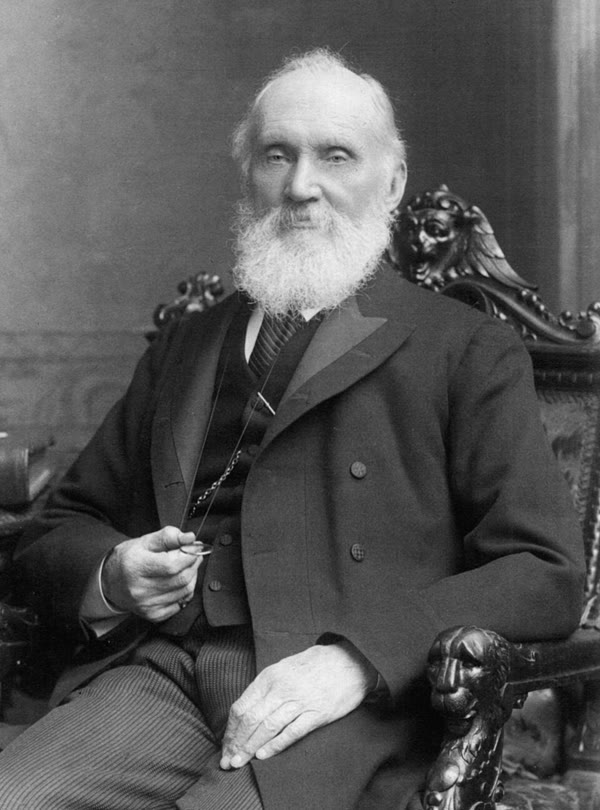
\includegraphics[height=5.2cm]{images/book2/g12-kelvin-1906.jpg}

{\small William Thomson, lorde Kelvin, em 1906. Fotografia Russell and Sons,
Londres (Smithsonian Institution Libraries, sem restrições de direitos
autorais conhecidas).}
\end{omfigure}
% ledger: photo:g12-kelvin

\begin{recall}
A datação relativa põe as rochas e os eventos em ordem; uma idade absoluta é
um número de anos (Livro 1, 7º ano). Um isótopo radioativo, o pai, decai
num isótopo filho ao acaso: o número $N$ de átomos pais que restam cai como
$N = N_0\,e^{-\lambda t}$, em que $\lambda$ é a constante de decaimento, e se
reduz à metade a cada meia-vida $T = \ln 2/\lambda$ (os livros de física).
Os minerais mais antigos conhecidos, zircões da Austrália Ocidental, têm 4.4
bilhões de anos (\cref{ch:g12:continental-crust}). A Terra também perde um
calor que a radioatividade continua a produzir, e o seu manto convecta
(\cref{ch:g12:internal-heat}).
\end{recall}
% ledger: wilde01:zircon

\section{Uma história das estimativas}

Antes da radioatividade, toda estimativa da \omterm{def:g12:age-of-the-earth:age}{idade da Terra} se apoiava num
processo cuja taxa se supunha conhecida.

\begin{center}
\small
\begin{tabular}{|p{0.19\linewidth}|p{0.42\linewidth}|p{0.25\linewidth}|}
\hline
quem, quando & método e o que ele supõe & estimativa \\
\hline
Phillips, 1860 & espessura das camadas sedimentares dividida por uma taxa de deposição; supõe uma taxa constante & de 38 a 96 milhões de anos \\
Kelvin, 1862 & resfriamento de uma Terra fundida só por condução, sem nenhuma fonte de calor no interior & de 20 a 400 milhões de anos \\
G.\,H.~Darwin & tempo desde que a Lua se separou da Terra, a partir da desaceleração dos seus movimentos pelas marés & pelo menos 56 milhões de anos \\
Joly, 1899 & sal levado ao mar pelos rios, dividido pelo aporte anual; supõe um aporte constante e nenhum sal removido & de 80 a 100 milhões de anos \\
\hline
\end{tabular}
\end{center}
% ledger: holmes13:estimates

\begin{history}[O calor que faltava a Kelvin]
Em 1903, Pierre Curie e Albert Laborde mostraram que o rádio libera calor, e
vários cientistas logo argumentaram que esse calor derrubava a conclusão de
Kelvin. Um ano depois, Ernest Rutherford, numa conferência com Kelvin na
plateia, lembrou-lhe que ele tinha limitado a \omterm{def:g12:age-of-the-earth:age}{idade da Terra} ``desde que
nenhuma nova fonte de calor fosse descoberta''. A radioatividade parecia ser
essa fonte. No entanto, não era o principal erro de Kelvin: o que mais
prolonga o resfriamento da Terra é a \omterm{def:g12:internal-heat:convection}{convecção do manto}, que mantém o manto
superior quente e o gradiente na crosta alto por muito mais tempo do que a
condução sozinha manteria.
\end{history}
% ledger: england:kelvin (Book 3 row)

A radioatividade também deu um relógio. Em 1907, Bertram Boltwood mostrou
que minerais de urânio da mesma idade contêm a mesma quantidade de chumbo
para cada grama de urânio: o chumbo é produzido pelo urânio. Em 1913, Arthur
Holmes podia escrever que as rochas mais antigas datadas tinham \num{1600}
milhões de anos, e em 1927 ele situou a \omterm{def:g12:age-of-the-earth:age}{idade da Terra} entre 1.6 e 3.0
bilhões de anos. Em 1956, Clair Patterson mediu 4.55 bilhões de anos. O
valor de hoje é 4.54 bilhões de anos, com uma margem de um por cento.
% ledger: holmes13:estimates, holmes27:age, patterson56:table, usgs:age-earth (Book 1 row)

\begin{omfigure}
\begin{tikzpicture}
\begin{axis}[omrecord, width=0.78\linewidth, height=6.2cm, ymode=log, xmin=1840, xmax=2040,
  ymin=1e7, ymax=2e10, xlabel={ano da estimativa}, ylabel={idade estimada da Terra (anos)},
  xtick={1850,1875,...,2025}, x tick label style={/pgf/number format/.cd, set thousands separator={}},
  ytick={1e7,1e8,1e9,1e10}, ymajorgrids=true, xmajorgrids=false]
% computed in figdata/grade-12/isochrons.py; ledger: holmes13:estimates, holmes27:age, patterson56:table, usgs:age-earth (Book 1 row)
\addplot[omDef, only marks, mark=*, mark size=1.8pt, error bars/.cd, y dir=both, y explicit]
  table[x=year, y=mid, y error minus expr=\thisrow{mid}-\thisrow{lo}, y error plus expr=\thisrow{hi}-\thisrow{mid}]
  {figdata/out/grade-12-isochrons-history.dat};
\addplot[omThm, densely dashed, domain=1840:2040, samples=2] {4.54e9};
\coordinate (k62) at (axis cs:1862,2.4e8);
\coordinate (k97) at (axis cs:1897,2.8e7);
\coordinate (jol) at (axis cs:1899,1e8);
\coordinate (h11) at (axis cs:1919,1.3e9);
\coordinate (pat) at (axis cs:1956,4.55e9);
\coordinate (now) at (axis cs:1845,4.54e9);
\end{axis}
\node[font=\scriptsize, anchor=west] at ([xshift=4pt]k62) {Kelvin 1862};
\node[font=\scriptsize, anchor=east] at ([xshift=-4pt]k97) {Kelvin 1897};
\node[font=\scriptsize, anchor=west] at ([xshift=4pt]jol) {Joly};
\node[font=\scriptsize, anchor=north] at (h11) {Holmes};
\node[font=\scriptsize, anchor=north west] at ([xshift=2pt, yshift=-3pt]pat) {Patterson};
\node[font=\scriptsize, text=omThm, anchor=south west] at (now) {hoje, 4.54 bilhões de anos};
\end{tikzpicture}

{\small Estimativas da \omterm{def:g12:age-of-the-earth:age}{idade da Terra} em função do ano em que foram feitas,
em escala logarítmica; as barras cobrem a faixa que cada autor deu. O ponto
de Holmes de 1913 é a idade das rochas mais antigas então datadas, um
mínimo. Fontes: Holmes (1913, 1927); Patterson (1956); U.S. Geological
Survey.}
\end{omfigure}

\section{Um relógio radioativo}

Um relógio radioativo só funciona se nada lhe foi acrescentado nem retirado
desde que ele começou a funcionar.

\begin{definition}[Sistema fechado]\label{def:g12:age-of-the-earth:closed-system}
Uma rocha ou um mineral é um \emph{sistema fechado}\index{sistema fechado}
para um isótopo pai e o seu filho se, desde o momento em que o seu relógio
começou, nenhum átomo do pai ou do filho entrou nele ou saiu dele, a não ser
pelo decaimento do pai no filho.
\end{definition}
% ledger: tulane:radiometric

Para um mineral, o relógio começa quando ele se cristaliza a partir de um
magma, ou, mais exatamente, quando ele esfriou o bastante para que os átomos
parem de entrar e sair dele. Um aquecimento, um fluido quente
ou o intemperismo podem abrir de novo o sistema, e a idade medida então
está errada, ou data esse evento posterior.
% ledger: tulane:radiometric

Contar os átomos filhos num \omterm{def:g12:age-of-the-earth:closed-system}{sistema fechado} dá a idade, desde que se saiba
quantos havia no início. Em geral, não se sabe. O rubídio-87 decai em
estrôncio-87, mas todo mineral também incorporou algum estrôncio-87 quando
se formou. O método da \omterm{def:g12:age-of-the-earth:isochron}{isócrona} contorna isso medindo vários minerais de uma
mesma rocha.

\section{A isócrona}

O estrôncio tem um isótopo, o estrôncio-86, que é estável e não é produzido
por nenhum decaimento: num \omterm{def:g12:age-of-the-earth:closed-system}{sistema fechado}, o seu número continua o mesmo, e
ele serve de referência. As razões isotópicas $^{87}\mathrm{Sr}/^{86}\mathrm{Sr}$ e
$^{87}\mathrm{Rb}/^{86}\mathrm{Sr}$ são o que um espectrômetro de massa mede.

\begin{theorem}[A equação da isócrona]\label{thm:g12:age-of-the-earth:isochron}
Num mineral que foi um \omterm{def:g12:age-of-the-earth:closed-system}{sistema fechado} durante um tempo $t$,
\[
  \left(\frac{^{87}\mathrm{Sr}}{^{86}\mathrm{Sr}}\right)_{\text{agora}}
  = \left(\frac{^{87}\mathrm{Sr}}{^{86}\mathrm{Sr}}\right)_{0}
  + \left(\frac{^{87}\mathrm{Rb}}{^{86}\mathrm{Sr}}\right)_{\text{agora}}
  \left(e^{\lambda t} - 1\right),
\]
em que o índice 0 marca o valor quando o relógio começou e $\lambda$ é a
constante de decaimento do rubídio-87.
\end{theorem}

\begin{proof}
Seja $P$ o número de átomos de rubídio-87 agora e $P_0$ quando o relógio
começou. Pela lei do decaimento, $P = P_0\,e^{-\lambda t}$, logo $P_0 = P\,e^{\lambda t}$,
e o número de átomos que decaíram é $P_0 - P = P\,(e^{\lambda t}-1)$.
Num \omterm{def:g12:age-of-the-earth:closed-system}{sistema fechado}, cada um deles virou um átomo de estrôncio-87, que se
soma aos $D_0$ átomos presentes no início: $D = D_0 + P\,(e^{\lambda
t}-1)$. Dividindo pelo número de átomos de estrôncio-86, que não mudou,
obtém-se a equação.
\end{proof}
% ledger: tulane:radiometric

Os minerais de um granito se cristalizaram a partir de um mesmo magma, então
todos começaram com a mesma razão $(^{87}\mathrm{Sr}/^{86}\mathrm{Sr})_0$.
Mas eles incorporaram quantidades muito diferentes de rubídio. Todos
compartilham o mesmo $t$ e a mesma razão inicial, então a equação diz que os
seus pontos ficam sobre uma mesma reta.

\begin{definition}[Isócrona]\label{def:g12:age-of-the-earth:isochron}
Uma \emph{isócrona}\index{isocrona@isócrona} é a reta sobre a qual ficam os
pontos de minerais ou de rochas que se formaram ao mesmo tempo a partir da
mesma fonte e continuaram \omterm{def:g12:age-of-the-earth:closed-system}{sistemas fechados} desde então, quando a razão do
filho para o isótopo estável é representada em função da razão do pai para o
isótopo estável. A sua inclinação dá a idade deles, e o ponto em que ela
encontra o eixo vertical dá a sua razão inicial.
\end{definition}
% ledger: tulane:radiometric

\begin{proposition}[A idade a partir da inclinação]\label{prop:g12:age-of-the-earth:slope}
Se uma \omterm{def:g12:age-of-the-earth:isochron}{isócrona} tem inclinação $m$, a idade é
\[
  t = \frac{\ln(1+m)}{\lambda}.
\]
\end{proposition}

\begin{proof}
Comparando com a equação da \omterm{def:g12:age-of-the-earth:isochron}{isócrona}, $m = e^{\lambda t} - 1$, logo
$e^{\lambda t} = 1 + m$, $\lambda t = \ln(1+m)$, e $t = \ln(1+m)/\lambda$.
\end{proof}

Para o rubídio-87, $\lambda = \num{1.3972e-11}$ por ano, uma meia-vida de
$\ln 2/\lambda \approx 49.6$ bilhões de anos: mais de dez vezes a \omterm{def:g12:age-of-the-earth:age}{idade da
Terra}.
% ledger: villa22:rb87

\begin{method}[Datar uma rocha com uma isócrona]\label{met:g12:age-of-the-earth:isochron}
\begin{enumerate}
  \item Separe vários minerais da rocha (ou tome várias amostras dela) com
        quantidades diferentes de rubídio.
  \item Meça em cada um as razões $^{87}\mathrm{Rb}/^{86}\mathrm{Sr}$ ($x$)
        e $^{87}\mathrm{Sr}/^{86}\mathrm{Sr}$ ($y$).
  \item Represente $y$ em função de $x$ e verifique que os pontos ficam
        sobre uma reta: se um não fica, essa amostra não foi um \omterm{def:g12:age-of-the-earth:closed-system}{sistema
        fechado}.
  \item Tome a inclinação $m$ da reta, e calcule $t = \ln(1+m)/\lambda$.
  \item Leia a razão inicial onde a reta encontra o eixo vertical.
\end{enumerate}
\end{method}

\begin{example}[O granito de Varden]\label{ex:g12:age-of-the-earth:varden}
O granito das Colinas de Varden, a região inventada desta série, dá estas
razões (dados de exercício):
\begin{center}
\small
\begin{tabular}{|l|c|c|}
\hline
amostra & $^{87}\mathrm{Rb}/^{86}\mathrm{Sr}$ & $^{87}\mathrm{Sr}/^{86}\mathrm{Sr}$ \\
\hline
plagioclásio & 0.35 & 0.70952 \\
hornblenda  & 1.20 & 0.71321 \\
rocha total  & 3.10 & 0.72146 \\
feldspato potássico  & 6.40 & 0.73578 \\
biotita     & 24.0 & 0.81218 \\
\hline
\end{tabular}
\end{center}
Passando pelo plagioclásio e pela biotita, a inclinação é
$m = (0.81218 - 0.70952)/(24.0 - 0.35) \approx 0.004341$. Então
$t = \ln(1.004341)/\num{1.3972e-11} \approx \num{3.10e8}$ anos:
o granito tem 310 milhões de anos. A reta encontra o eixo vertical em
$0.70952 - 0.35 \times 0.004341 \approx 0.7080$, a razão inicial.
\end{example}
% values: granite_age_Ma 310.0, granite_intercept 0.70800 (isochrons.py)

\begin{omfigure}
\begin{tikzpicture}
\begin{axis}[omrecord, width=0.7\linewidth, height=6cm, xmin=0, xmax=26, ymin=0.695, ymax=0.82, ytick={0.70,0.72,...,0.82},
  xlabel={$^{87}\mathrm{Rb}/^{86}\mathrm{Sr}$}, ylabel={$^{87}\mathrm{Sr}/^{86}\mathrm{Sr}$},
  y tick label style={/pgf/number format/.cd, fixed, fixed zerofill, precision=2}]
% computed in figdata/grade-12/isochrons.py (exercise data, Varden granite 310 Ma); ledger: villa22:rb87
\addplot[omDef, line width=0.9pt] table[x=x, y=y] {figdata/out/grade-12-isochrons-graniteln.dat};
\addplot[omThm, only marks, mark=*, mark size=2pt] table[x=rbsr, y=srsr] {figdata/out/grade-12-isochrons-granite.dat};
\addplot[black!60, densely dotted, domain=0:26, samples=2] {0.7080};
\coordinate (pl) at (axis cs:0.35,0.70952);
\coordinate (hb) at (axis cs:1.2,0.71321);
\coordinate (wr) at (axis cs:3.1,0.72146);
\coordinate (kf) at (axis cs:6.4,0.73578);
\coordinate (bt) at (axis cs:24,0.81218);
\coordinate (sl) at (axis cs:12,0.762);
\coordinate (in) at (axis cs:9,0.7082);
\coordinate (plhb) at (axis cs:0.6,0.737);
\coordinate (plhbpt) at (axis cs:0.9,0.7125);
\end{axis}
\node[font=\scriptsize, anchor=north west] at ([xshift=1pt]wr) {rocha total};
\node[font=\scriptsize, anchor=north west] at ([xshift=1pt]kf) {feldspato potássico};
\node[font=\scriptsize, anchor=east] at ([xshift=-3pt]bt) {biotita};
\node[font=\scriptsize, anchor=south west, align=left, inner sep=1pt] (plhblab) at (plhb) {plagioclásio,\\hornblenda};
\draw[black!60, line width=0.4pt] (plhblab.south) -- (plhbpt);
\node[font=\scriptsize, text=omDef, anchor=south east] at (sl) {\shortstack[r]{inclinação $0.004341$:\\310 milhões de anos}};
\node[font=\scriptsize, text=black!70, anchor=south west] at (in) {razão inicial 0.7080 (tempo 0)};
\end{tikzpicture}

{\small A \omterm{def:g12:age-of-the-earth:isochron}{isócrona} rubídio--estrôncio do granito de Varden (dados de
exercício). Quando o granito se formou, todos os seus minerais ficavam sobre
a reta horizontal pontilhada; desde então, cada um subiu em proporção ao seu
rubídio, e hoje eles ficam sobre a reta contínua.}
\end{omfigure}

\begin{inthelab}[Pesar átomos]
As razões são medidas com um espectrômetro de massa. Alguns miligramas de um
mineral são dissolvidos em ácido, e o estrôncio é separado do rubídio por
via química, já que os dois isótopos de massa 87 seriam contados juntos de
outro modo. O estrôncio, depositado sobre um filamento de metal e aquecido
no vácuo, emite íons; um campo elétrico os acelera e um ímã curva as suas
trajetórias, os íons mais leves mais que os mais pesados, de modo que cada
isótopo chega ao seu próprio coletor. As suas correntes dão as razões.
\end{inthelab}

\begin{omfigure}
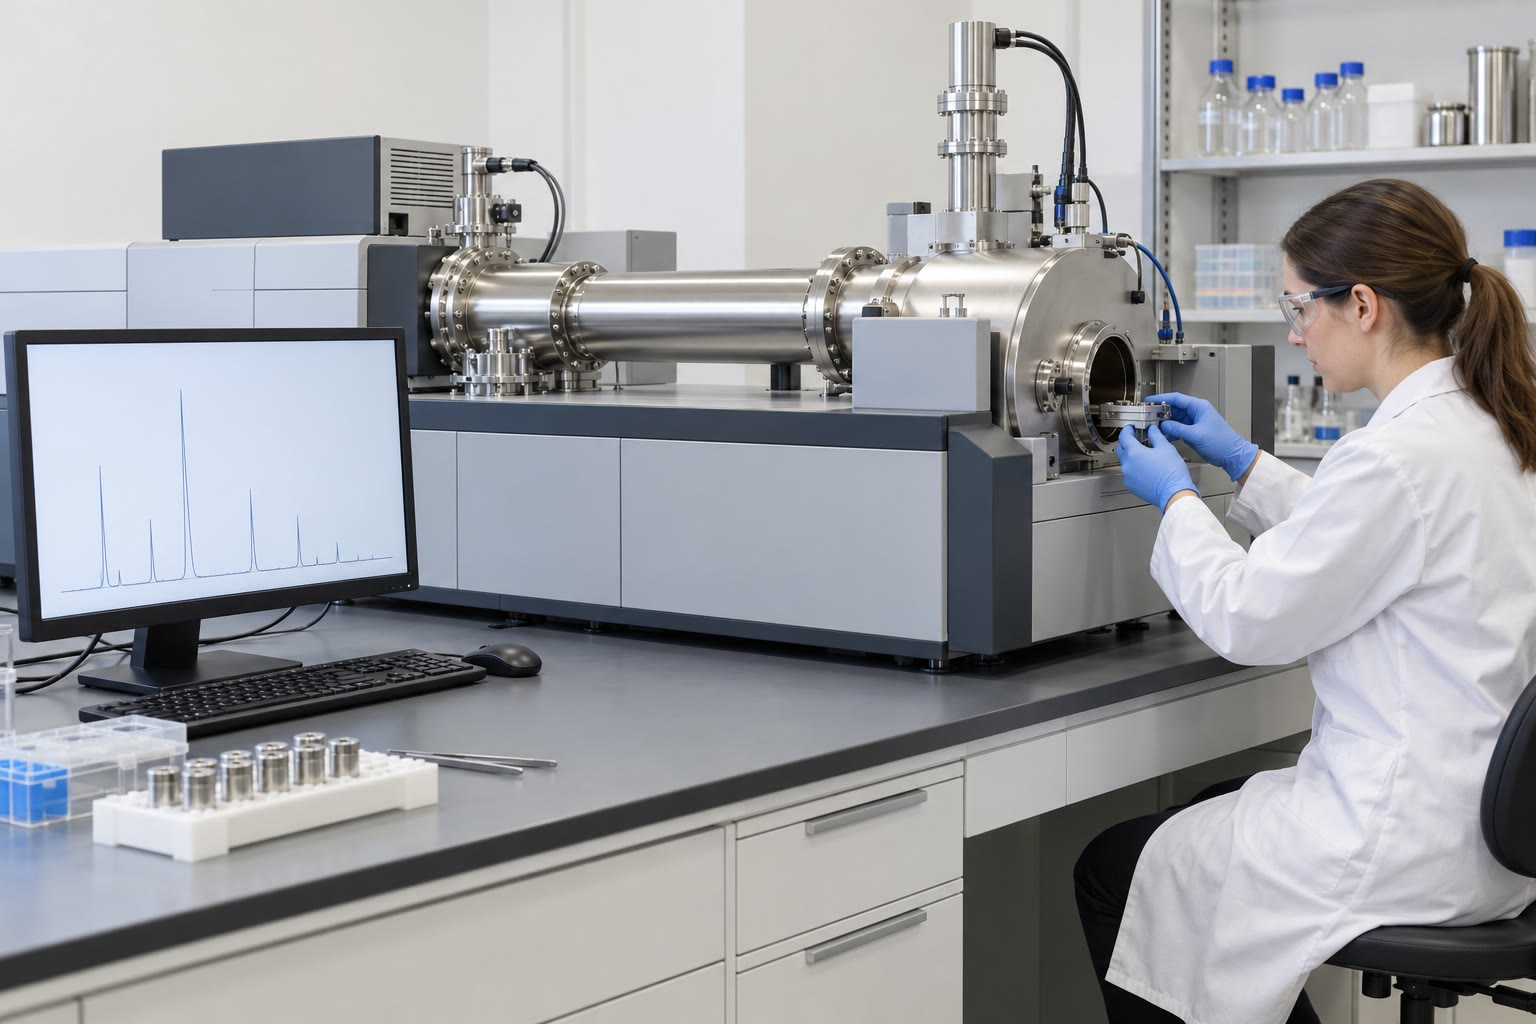
\includegraphics[width=0.66\linewidth]{images/book2/ai/g12-mass-spectrometer-lab.jpg}

{\small Um espectrômetro de massa num laboratório: uma amostra está sendo
carregada na extremidade da fonte. Ilustração gerada por IA.}
\end{omfigure}

A razão inicial é também um indício da origem do magma. O rubídio prefere o
líquido quando o manto se funde, então ao longo das eras ele se concentrou
na \omterm{def:g12:continental-crust:continental-crust}{crosta continental}, que produziu por isso mais estrôncio-87: as rochas
da crosta têm uma razão $^{87}\mathrm{Sr}/^{86}\mathrm{Sr}$ mais alta
que as rochas do manto. Um magma formado por fusão da crosta herda essa
razão alta.
% ledger: tulane:radiometric

\section{A idade da Terra}

Nenhuma rocha da Terra remonta ao início da Terra: a rocha mais antiga
conhecida, o gnaisse de Acasta, tem 4.03 bilhões de anos, e os zircões mais
antigos 4.4 bilhões. A superfície foi fundida, erodida e reciclada desde
então. A datação da própria Terra vem dos meteoritos, fragmentos dos
pequenos corpos que se formaram com os planetas e alguns dos quais
continuaram \omterm{def:g12:age-of-the-earth:closed-system}{sistemas fechados} desde então.
% ledger: bowring99:acasta, wilde01:zircon, usgs:age-earth (Book 1 row)

\begin{definition}[Idade da Terra]\label{def:g12:age-of-the-earth:age}
A \emph{idade da Terra}\index{idade da Terra} é o tempo desde que a Terra se
formou pela acreção de corpos menores, no nascimento do Sistema Solar.
Medida a partir dos meteoritos por datação radiométrica, ela é de
\num{4.54} bilhões de anos, com uma margem de um por cento.
\end{definition}
% ledger: usgs:age-earth (Book 1 row)

Em 1956, Clair Patterson mediu os isótopos do chumbo em três meteoritos
rochosos e dois meteoritos metálicos. Dois isótopos do chumbo são produzidos
pelo decaimento do urânio, o chumbo-206 a partir do urânio-238 e o
chumbo-207 a partir do urânio-235, enquanto o chumbo-204 não é produzido
por nenhum decaimento. Como no caso do estrôncio, os pontos dos meteoritos
que se formaram ao mesmo tempo ficam sobre uma reta, quando
$^{207}\mathrm{Pb}/^{204}\mathrm{Pb}$ é representado em função de
$^{206}\mathrm{Pb}/^{204}\mathrm{Pb}$. O meteorito metálico de Canyon
Diablo, no Arizona, quase não contém urânio: o seu chumbo não mudou desde
que ele se formou, e marca a extremidade inferior da reta, o chumbo com que
o Sistema Solar começou.
% ledger: patterson56:table, patterson56:constants, usgs:age-earth (Book 1 row: Canyon Diablo troilite)

\begin{omfigure}
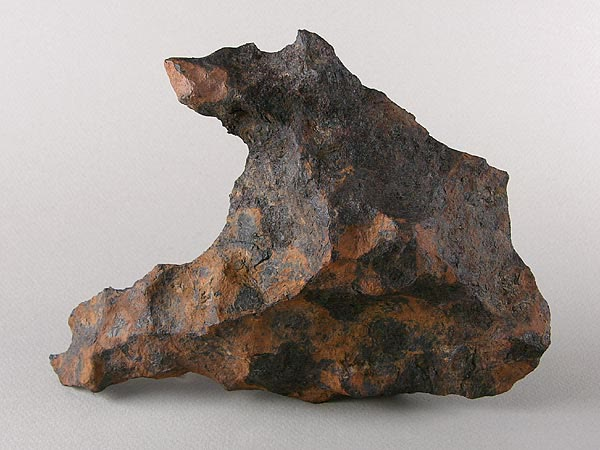
\includegraphics[height=4.2cm]{images/book2/g12-canyon-diablo-meteorite.jpg}

{\small Um fragmento do meteorito metálico de Canyon Diablo, \qty{2641}{g}.
Fotografia Geoffrey Notkin, CC~BY-SA~2.5 (Wikimedia Commons).}
\end{omfigure}
% ledger: photo:g12-canyon-diablo

Para o chumbo, a inclinação $m$ depende da idade através dos dois isótopos
do urânio; a relação é admitida aqui. Com as constantes que Patterson usou,
\[
  m = \frac{1}{137.8}\,\frac{e^{\lambda_{235}t}-1}{e^{\lambda_{238}t}-1},
  \qquad \lambda_{235} = \num{9.72e-10},\ \lambda_{238} = \num{1.537e-10}
  \text{ por ano},
\]
o que dá:
\begin{center}
\small
\begin{tabular}{|l|c|c|c|c|c|c|}
\hline
idade (bilhões de anos) & 4.40 & 4.45 & 4.50 & 4.55 & 4.60 & 4.65 \\
inclinação $m$ & 0.533 & 0.551 & 0.570 & 0.590 & 0.610 & 0.632 \\
\hline
\end{tabular}
\end{center}
% ledger: patterson56:constants
% values: pb_slope at 4.40-4.65 Ga (isochrons.py pb_slope)

\begin{omfigure}
\begin{tikzpicture}
\begin{axis}[omrecord, width=0.72\linewidth, height=6cm, xmin=0, xmax=56, ymin=0, ymax=40,
  xlabel={$^{206}\mathrm{Pb}/^{204}\mathrm{Pb}$}, ylabel={$^{207}\mathrm{Pb}/^{204}\mathrm{Pb}$}]
% computed in figdata/grade-12/isochrons.py; ledger: patterson56:table
\addplot[omDef, line width=0.9pt] table[x=x, y=y] {figdata/out/grade-12-isochrons-pbln.dat};
\addplot[omThm, only marks, mark=*, mark size=2pt] table[x=r206, y=r207, restrict expr to domain={\thisrow{idx}}{1:5}] {figdata/out/grade-12-isochrons-pbpb.dat};
\addplot[black, only marks, mark=o, mark size=2.6pt, line width=0.8pt] table[x=r206, y=r207, restrict expr to domain={\thisrow{idx}}{6:6}] {figdata/out/grade-12-isochrons-pbpb.dat};
\coordinate (nl) at (axis cs:50.28,34.86);
\coordinate (fc) at (axis cs:19.48,15.76);
\coordinate (cd) at (axis cs:9.5,10.36);
\coordinate (sed) at (axis cs:19.0,15.5);
\coordinate (sl) at (axis cs:30,25);
\end{axis}
\node[font=\scriptsize, anchor=north west] at ([xshift=2pt]nl) {Nuevo Laredo};
\node[font=\scriptsize, anchor=north west, align=left] at ([xshift=4pt, yshift=-2pt]fc) {Forest City, Modoc;\\sedimento oceânico (círculo)};
\node[font=\scriptsize, anchor=north west, align=left] at ([xshift=3pt, yshift=-3pt]cd) {Canyon Diablo, Henbury (metálicos)};
\node[font=\scriptsize, text=omDef, anchor=south east] at (sl) {\shortstack[r]{inclinação 0.603:\\cerca de 4.6 bilhões de anos}};
\end{tikzpicture}

{\small A \omterm{def:g12:age-of-the-earth:isochron}{isócrona} do chumbo de Patterson: os cinco meteoritos ficam sobre
uma mesma reta, e quase também o chumbo de um sedimento oceânico moderno,
que representa a Terra. Fonte: Patterson (1956), Tabela~1.}
\end{omfigure}
% values: pb_slope 0.6026, pb_age_Ga 4.58, sediment_residual -0.39 (isochrons.py)

Uma reta traçada pelos cinco pontos tem uma inclinação de cerca de 0.603,
entre as inclinações para 4.55 e 4.60 bilhões de anos da tabela. O
resultado do próprio Patterson, levando em conta os erros das medições e das
constantes de decaimento, foi de 4.55 bilhões de anos, com uma margem de
0.07. Ele mediu depois o chumbo de um sedimento oceânico moderno, que mistura
chumbo de uma grande massa da crosta da Terra: ele fica sobre a mesma reta.
O chumbo da Terra evoluiu como o dos meteoritos, ao longo do mesmo tempo: a
Terra é tão antiga quanto eles.
% ledger: patterson56:table

Desde então, centenas de medições o confirmaram. Os meteoritos dão idades de
4.53 a 4.58 bilhões de anos, e os sólidos mais antigos do Sistema Solar,
pequenas inclusões ricas em cálcio e alumínio encontradas em alguns
meteoritos, se formaram há \num{4567.30} milhões de anos, com uma margem de
0.16. A Terra se formou mais tarde a partir desse material, e é por isso que
a sua idade, 4.54 bilhões de anos, é um pouco menor que a deles.
% ledger: usgs:age-earth (Book 1 row), connelly12:cai

\section{Exercícios}

\begin{exercise}[$\star$]\label{exo:g12:age-of-the-earth:1}
Dê a palavra: (a) um mineral em que nenhum átomo pai ou filho entrou ou do
qual nenhum saiu desde que o seu relógio começou; (b) a reta sobre a qual
ficam os minerais de uma mesma idade e de uma mesma fonte; (c) o tempo desde
que a Terra se formou por acreção.
\end{exercise}

\begin{exercise}[$\star$]\label{exo:g12:age-of-the-earth:2}
Usando a tabela do granito de Varden, ponha as suas cinco amostras na ordem
da sua razão de rubídio-87 para estrôncio-86, da mais baixa. Qual delas fica
mais alta na \omterm{def:g12:age-of-the-earth:isochron}{isócrona}, e por que ela produziu mais estrôncio-87?
\end{exercise}

\begin{exercise}[$\star$]\label{exo:g12:age-of-the-earth:3}
Calcule a meia-vida do rubídio-87 a partir da sua constante de decaimento,
\num{1.3972e-11} por ano. Quantas vezes a \omterm{def:g12:age-of-the-earth:age}{idade da Terra} ela vale?
\end{exercise}

\begin{exercise}[$\star$]\label{exo:g12:age-of-the-earth:4}
Calcule $e^{\lambda t} - 1$ para o rubídio-87 para $t = 310$ milhões de
anos e $t = 480$ milhões de anos.
\end{exercise}

\begin{exercise}[$\star$]\label{exo:g12:age-of-the-earth:5}
Ponha em ordem de data as estimativas de Phillips, Holmes (1927), Joly,
Kelvin (1862) e Patterson. Quantas vezes maior que o limite superior da
estimativa de Joly é a idade atual da Terra?
\end{exercise}

\begin{exercise}[$\star\star$]\label{exo:g12:age-of-the-earth:6}
Um mineral do granito de Varden (310 milhões de anos, razão inicial 0.7080)
tem $^{87}\mathrm{Rb}/^{86}\mathrm{Sr} = 10.0$. Qual é a sua
$^{87}\mathrm{Sr}/^{86}\mathrm{Sr}$ hoje? Qual era ela quando o granito se
formou?
\end{exercise}

\begin{exercise}[$\star\star$]\label{exo:g12:age-of-the-earth:7}
Quatro amostras do xisto de Varden dão $(x, y)$ = (0.90, 0.71806),
(2.60, 0.72950), (5.10, 0.74632) e (9.40, 0.77525), com $x =
{}^{87}\mathrm{Rb}/^{86}\mathrm{Sr}$ e $y = {}^{87}\mathrm{Sr}/^{86}\mathrm{Sr}$.
(1) A partir da primeira e da última amostras, calcule a inclinação e a
idade. (2) Verifique que as duas amostras do meio ficam sobre a mesma reta.
(3) O resultado é coerente com os 310 milhões de anos do granito e com o
princípio das relações de corte?
\end{exercise}

\begin{exercise}[$\star\star$]\label{exo:g12:age-of-the-earth:8}
Por que uma rocha em que todos os minerais têm a mesma razão de rubídio para
estrôncio não dá nenhuma \omterm{def:g12:age-of-the-earth:isochron}{isócrona}? Por que a biotita, no granito de Varden,
fixa a inclinação melhor que os outros minerais?
\end{exercise}

\begin{exercise}[$\star\star$]\label{exo:g12:age-of-the-earth:9}
Muito depois que o granito de Varden se formou, um fluido quente fez a sua
biotita perder parte do seu estrôncio-87. (1) Para onde o seu ponto se move
no diagrama da \omterm{def:g12:age-of-the-earth:isochron}{isócrona}? (2) Que idade a biotita e o plagioclásio sozinhos
dariam então: velha demais ou jovem demais? (3) Como o método da \omterm{def:g12:age-of-the-earth:isochron}{isócrona}
revela o problema?
\end{exercise}

\begin{exercise}[$\star\star$]\label{exo:g12:age-of-the-earth:10}
(1) Quantas vezes mais longa que os 96 milhões de anos de Kelvin é a \omterm{def:g12:age-of-the-earth:age}{idade
da Terra}? (2) Joly supôs que os rios levam sal ao mar a uma taxa constante e
que nada dele sai do mar. Qual dessas hipóteses torna a sua idade curta
demais se estiver errada, e por quê?
\end{exercise}

\begin{exercise}[$\star\star$]\label{exo:g12:age-of-the-earth:11}
Usando os valores de Patterson para Canyon Diablo (9.46, 10.34) e Nuevo
Laredo (50.28, 34.86), calcule a inclinação da reta que passa pelos dois
meteoritos, e leia a idade na tabela das inclinações.
\end{exercise}

\begin{exercise}[$\star\star\star$]\label{exo:g12:age-of-the-earth:12}
Um basalto da região de Varden, também com 310 milhões de anos, tem uma
razão inicial de 0.7035, contra 0.7080 para o granito. (1) Qual rocha tem
mais chance de vir do manto fundido, e qual da crosta fundida? (2) Explique
por quê com o que você sabe do rubídio. (3) As duas poderiam ter se
cristalizado a partir de um mesmo magma?
\end{exercise}

\begin{exercise}[$\star\star\star$]\label{exo:g12:age-of-the-earth:13}
(1) Que fração do rubídio-87 presente quando a Terra se formou resta hoje? E
do urânio-238 (meia-vida de 4.47 bilhões de anos)? (2) Qual seria a
inclinação de uma \omterm{def:g12:age-of-the-earth:isochron}{isócrona} rubídio--estrôncio para uma rocha de um milhão de
anos? Por que o rubídio--estrôncio é um relógio ruim para rochas jovens?
\end{exercise}

\begin{exercise}[$\star\star\star$]\label{exo:g12:age-of-the-earth:14}
A reta que passa pelos cinco meteoritos de Patterson é $y = 4.438 + 0.6026\,x$.
(1) Que $^{207}\mathrm{Pb}/^{204}\mathrm{Pb}$ ela prevê para o sedimento
oceânico, em $x = 19.0$? Patterson mediu 15.5: em que porcentagem eles
diferem? (2) Que idade a inclinação 0.6026 dá, pela tabela? Compare com os
$4.55 \pm 0.07$ bilhões de anos de Patterson.
\end{exercise}

\begin{exercise}[$\star\star\star$]\label{exo:g12:age-of-the-earth:15}
Kelvin supôs que todo o calor que a Terra perde, \qty{46.7}{TW} hoje, é
calor armazenado. (1) A radioatividade repõe cerca de \qty{24.4}{TW} dele.
Em quanto isso, sozinho, prolonga o tempo para perder uma dada reserva de
calor? (2) Partindo de 96 milhões de anos, isso basta para chegar à idade
verdadeira? (3) O que Kelvin deixou escapar que importa mais?
\end{exercise}

\begin{problem}[{Problema de fim de semana --- datar o granito de Varden}]
\label{pb:g12:age-of-the-earth:1}
% exercise data from figdata/grade-12/isochrons.py; ledger: villa22:rb87, tulane:radiometric, ics:base.Carboniferous, ics:base.Permian
O granito das Colinas de Varden, a região inventada desta série, corta o
xisto em volta dele. Um laboratório mediu cinco das suas amostras (exemplo
acima): plagioclásio (0.35, 0.70952), hornblenda (1.20, 0.71321), rocha
total (3.10, 0.72146), feldspato potássico (6.40, 0.73578) e biotita (24.0,
0.81218), cada uma como
$(^{87}\mathrm{Rb}/^{86}\mathrm{Sr},\ ^{87}\mathrm{Sr}/^{86}\mathrm{Sr})$. A
constante de decaimento do rubídio-87 é \num{1.3972e-11} por ano.

\medskip
\noindent\textbf{Parte I --- As amostras.}
\begin{enumerate}
  \item Que amostra é a mais rica em rubídio em relação ao estrôncio?
  \item Por que todos os minerais começaram com a mesma
        $^{87}\mathrm{Sr}/^{86}\mathrm{Sr}$?
  \item Por que as razões são tomadas em relação ao estrôncio-86?
  \item Qual dos três isótopos aumentou desde que o granito se formou, e por
        quê?
  \item Que aspecto tinham os cinco pontos no diagrama quando o granito
        acabava de se formar?
\end{enumerate}

\medskip
\noindent\textbf{Parte II --- A reta isócrona.}
\begin{enumerate}[resume]
  \item Calcule a inclinação pelo plagioclásio e pela biotita.
  \item Calcule a inclinação pelo plagioclásio e pela rocha total.
  \item Compare as duas inclinações. Qual é a mais confiável, e por quê?
  \item Encontre onde a reta da questão 6 encontra o eixo vertical.
  \item Verifique que o feldspato potássico fica sobre essa reta.
\end{enumerate}

\medskip
\noindent\textbf{Parte III --- A inclinação e a idade.}
\begin{enumerate}[resume]
  \item Escreva a relação entre a inclinação e $e^{\lambda t}$.
  \item Calcule $\lambda t$.
  \item Calcule a idade $t$.
  \item O xisto foi datado de 480 milhões de anos. A ordem das duas idades é
        a que as relações de campo exigem?
  \item O Carbonífero vai de 358.9 a 298.9 milhões de anos atrás. Em que
        período o granito se formou?
\end{enumerate}

\medskip
\noindent\textbf{Parte IV --- A razão inicial e a fonte.}
\begin{enumerate}[resume]
  \item O que representa a interseção, 0.7080?
  \item Um basalto da região se formou com uma razão de 0.7035. Qual rocha
        tem a razão inicial mais alta?
  \item Por que as rochas da crosta têm razões mais altas que o manto?
  \item O que a razão inicial do granito sugere sobre a rocha que se fundiu
        para formá-lo?
  \item Resuma: que idade tem o granito de Varden?
\end{enumerate}
\end{problem}
